% \setchapterstyle{kao}
\setchapterimage{chargers-title3}
\setchapterpreamble[u]{\margintoc}
\chapter{Data}
\label{ch:data}

\footnotetext{Title image is a map of Prague with all chargers denoted as triangles in available datasets. The layer below displays all buildings in Prague with color being the number of floors}



\textit{
    Mention all the available data forming our data landscape which determines whats possible. Those data are split into two groups. Target data which we would like to learn to predict. And then factors which we hypothesize that this data may explain our target variables.
    And also show it off. I am not sure if feature engineering fits into here.
}

\textit{Also talk about different data types. Spatial, temporal, spatio-temporal}


\section{EV Chargers and Charging Sessions}


\textit{Explanation of the charging sessions dataset. Chargers in Prague. Modelling assumption. And showing lots of pretty plots and pictures.}

\begin{figure}[hb]
    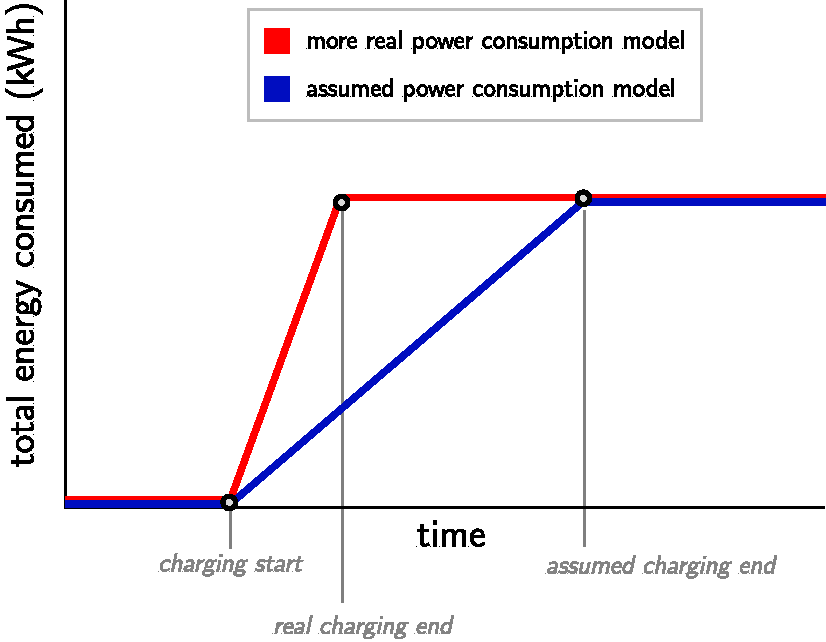
\includegraphics{charging-assumption.pdf}
    % \caption[Problem modelling overview]{Chapter content overview. }
\end{figure}

\section{Population numbers (ZSJ)}

\begin{figure}[hb]
    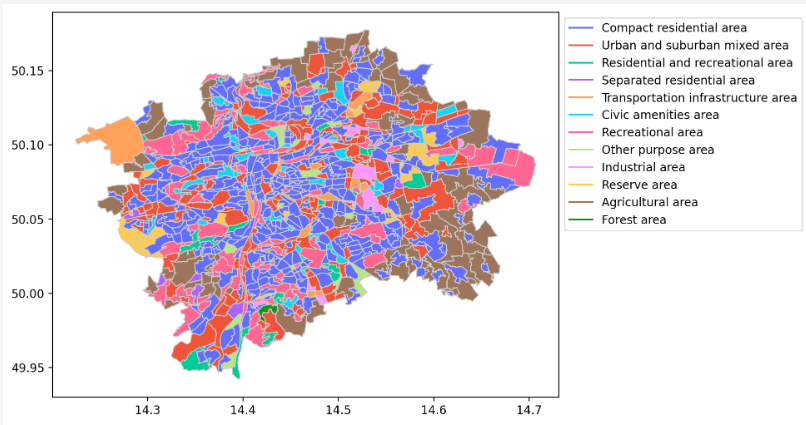
\includegraphics{zsj-type.png}
    % \caption[Problem modelling overview]{Chapter content overview. }
\end{figure}

\section{Points of Interest}


\section{People Mobility}

\begin{figure}[hb]
    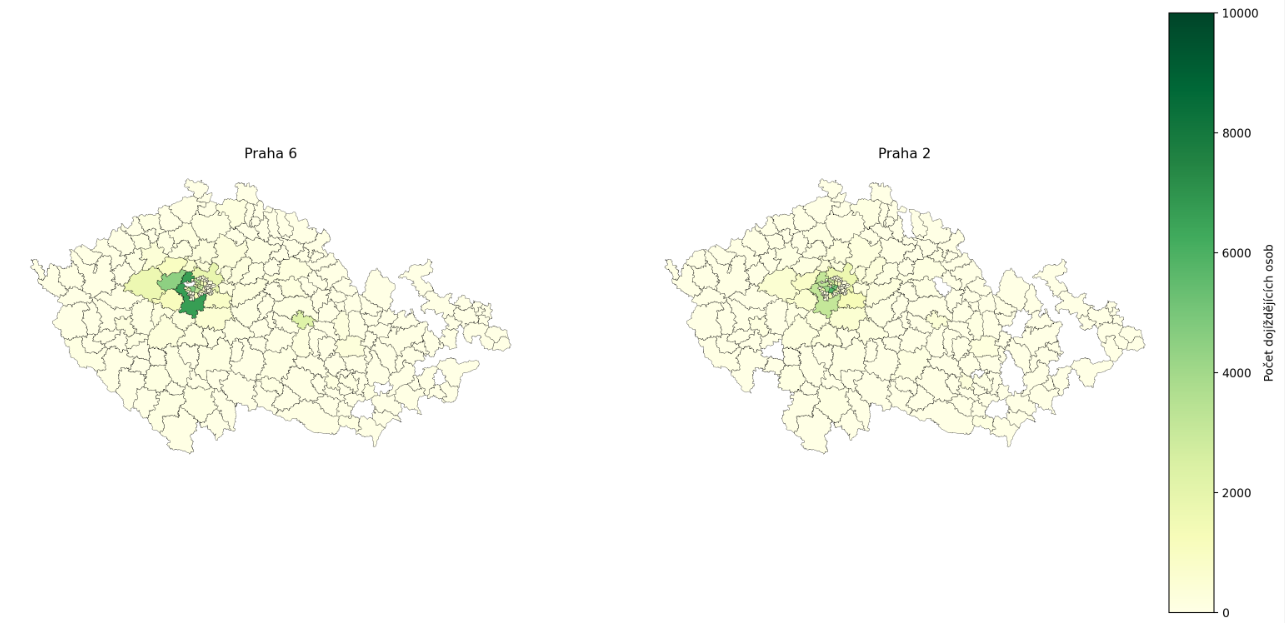
\includegraphics{commuting-people.png}
    \caption[Problem modelling overview]{Chapter content overview. }
\end{figure}

\section{Mobility Survey - cesko v pohybu}

\begin{figure}[hb]
    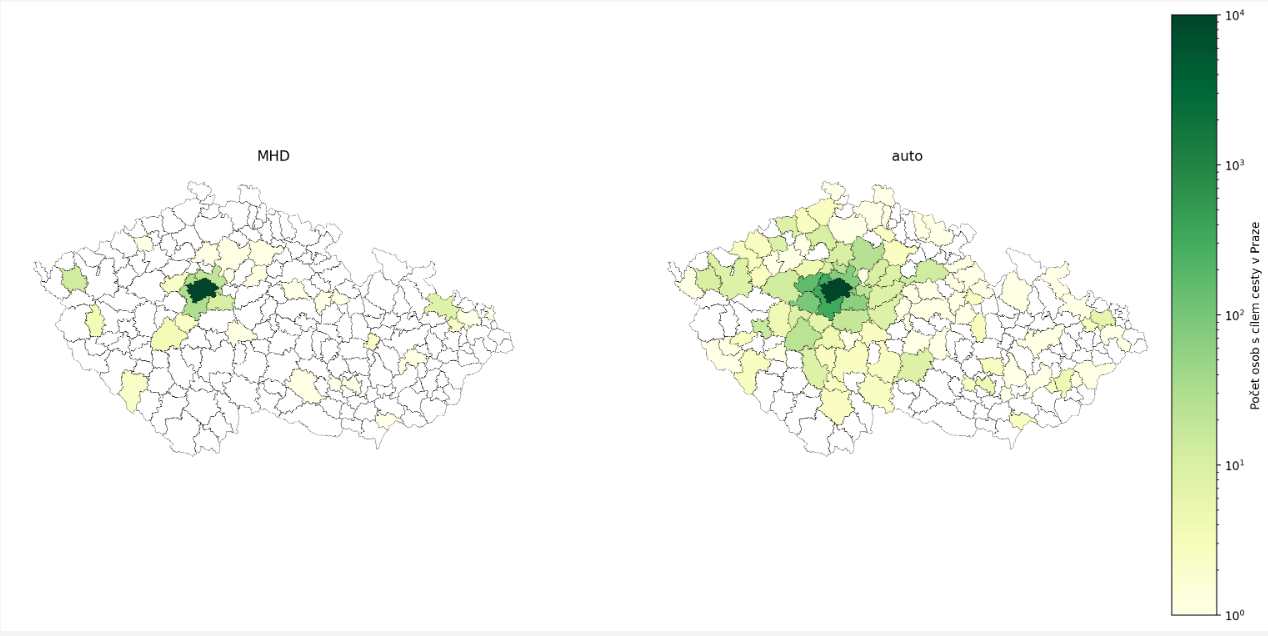
\includegraphics{vpohybu-trasnport-type.png}
    \caption[Problem modelling overview]{Chapter content overview. }
\end{figure}

---

Talks about what was extracted from datasets in \ref{ch:data}

\section{Spatial data}

\subsection{ZSJ Type and Population}

\subsection{Points of Interest}

Has statistically significant results for certain PoI \cite{hechtGlobalElectricVehicle2024}\cite{dongElectricVehicleCharging2019}
(\cite{dongElectricVehicleCharging2019} uses Gaussian cox model, \cite{hechtGlobalElectricVehicle2024} uses Neural networks and linear regression)

\cite{hechtGlobalElectricVehicle2024} states that radius of relevant PoIs is 2000metres. The research stated that the distance is sensible.
One solution is to just count all the PoIs in the radius but as they are more far away from the CP their relevance might decrease. The \cite{hechtGlobalElectricVehicle2024} thus uses importance factor for pair of PoI and CP.

$IF(PoI_i, CP_k) = max(r-d_{\text{sphere}}(PoI_i, CP_k),0)$


\subsubsection{Buildings (OsmPoisPbf)}


\subsubsection{Public Ammenities (OSMOX)}

how osmox works
\begin{figure}[hb]
    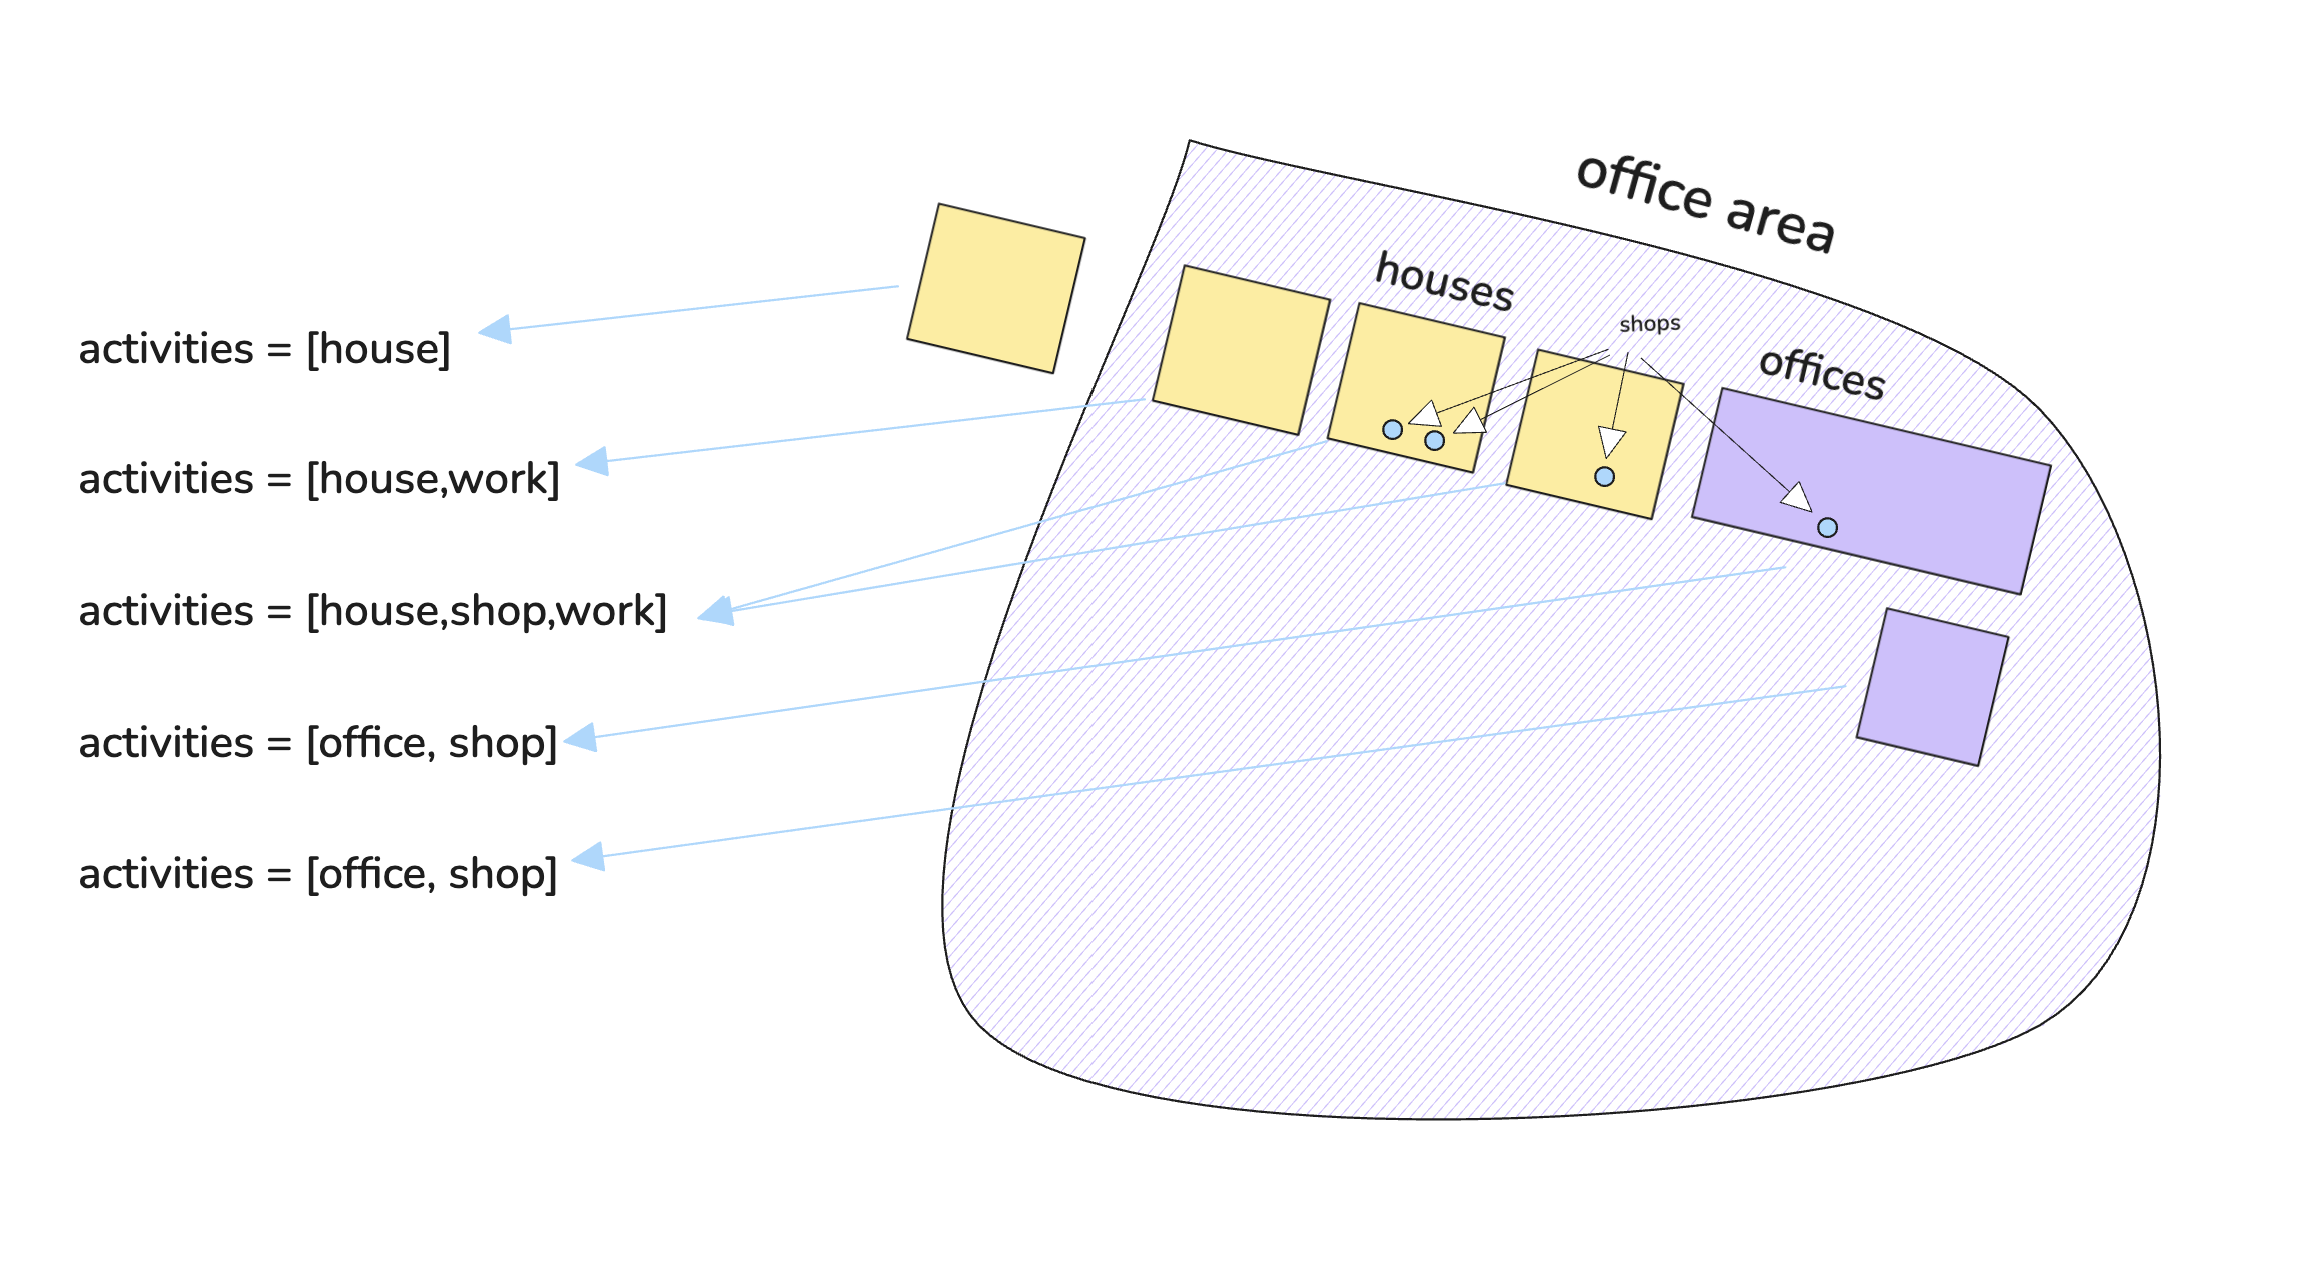
\includegraphics[width=0.7\textwidth]{osmox-poi.png}
    \caption[osmox]{osmox}
    \label{fig:nn-latent}
\end{figure}


\section{Charging profiles}


\begin{figure}[hb]
    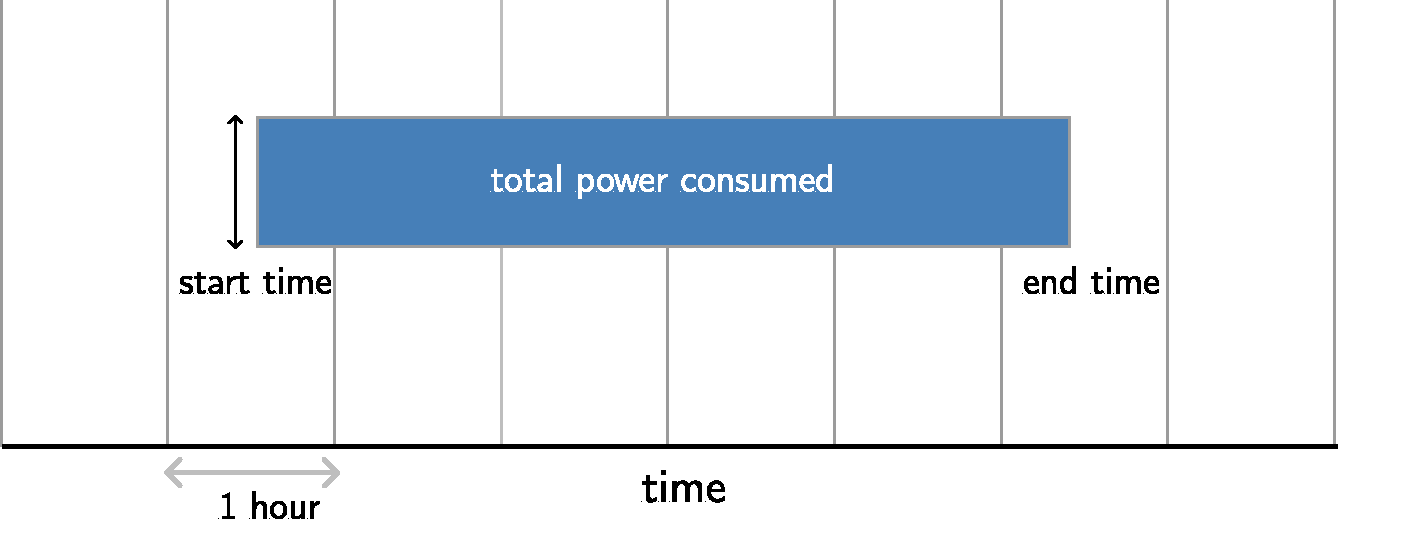
\includegraphics[width=0.7\textwidth]{cutting-1.pdf}
    % \caption[Cutting]{Cutting}
\end{figure}

\begin{figure}[hb]
    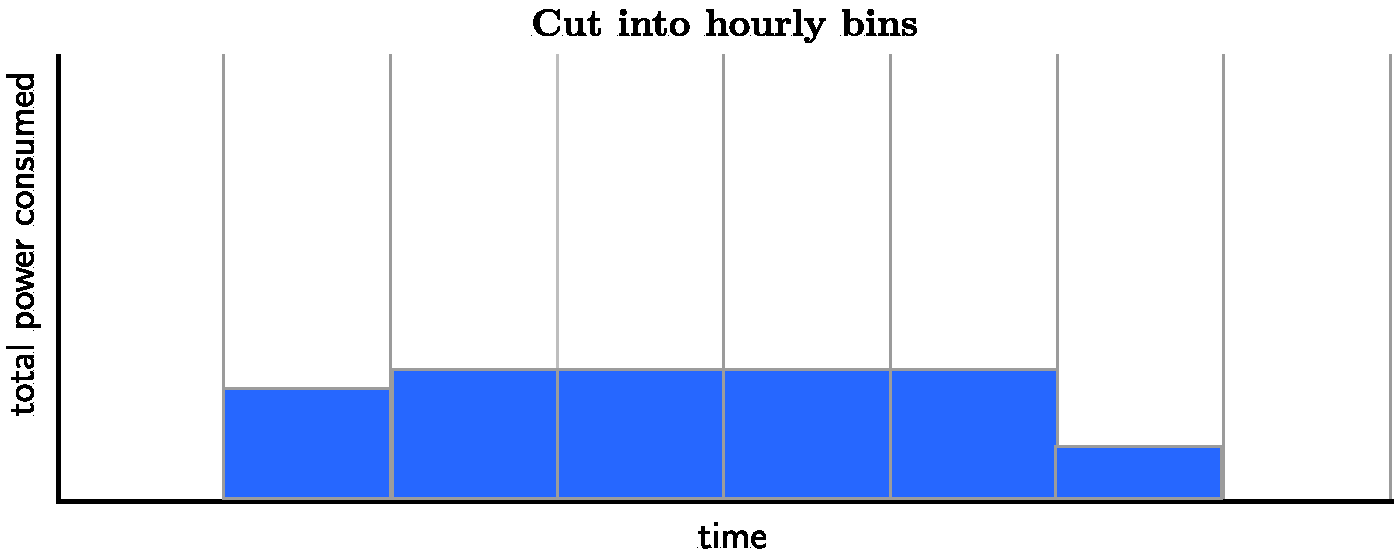
\includegraphics[width=0.7\textwidth]{cutting-2.pdf}
    % \caption[Cutting]{Cutting}
\end{figure}

\begin{figure}[hb]
    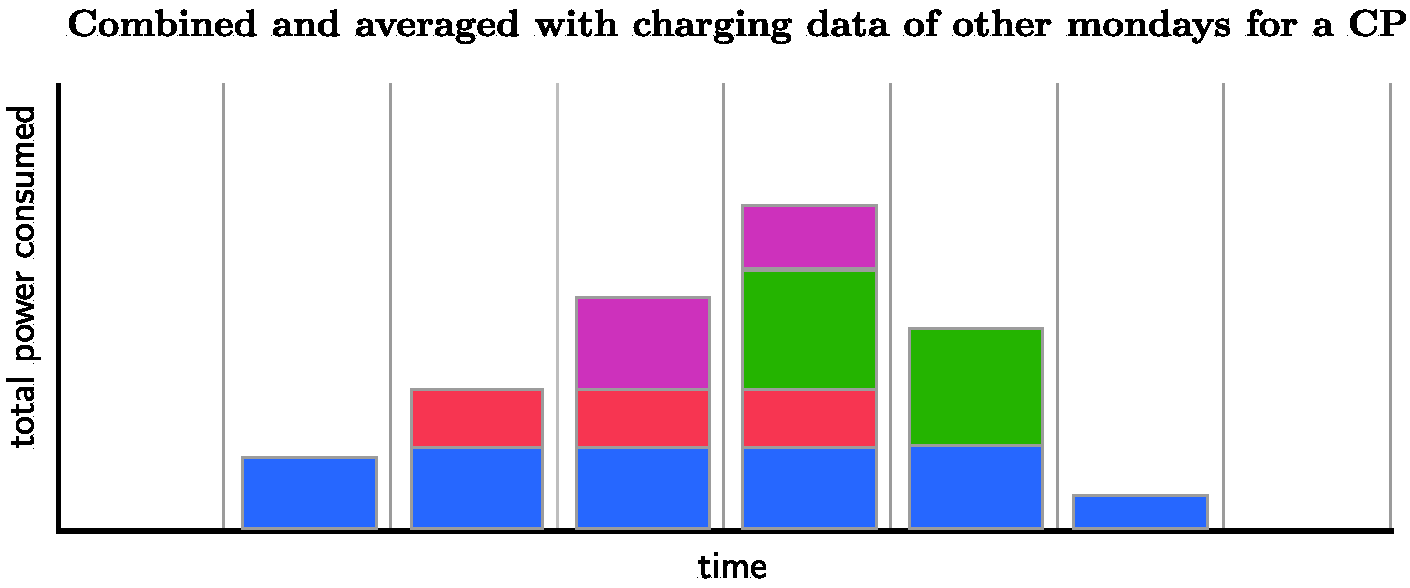
\includegraphics[width=0.7\textwidth]{cutting-3.pdf}
    % \caption[Cutting]{Cutting}
\end{figure}

